\section{Experimental}

%Characterize the system, give all details that matter. Describe how the experimental procedure went.

% CAS codes Hinzufügen?

\subsection{Chemicals}
The following experiments were conducted using ethanol (absolute $\geq$ \qty{99.8}{\percent}) and  ammonium nitrate (\qty{80.04}{\gram\per\mole}) ($\geq$ \qty{99}{\percent}) from \texttt{Sigma Aldrich} as well as commercially available apple cider vinegar purchased form the \texttt{Coop} supermarket chain. 

Additionally, a preprepared \qty{1}{\M} sodium hydroxide solution was used. Its origin and purity are unknown to the authors.

\subsection{Procedure}

A total of 5 experiments were prepared and carried out using the same setup.


\begin{figure}[H]
    \centering
    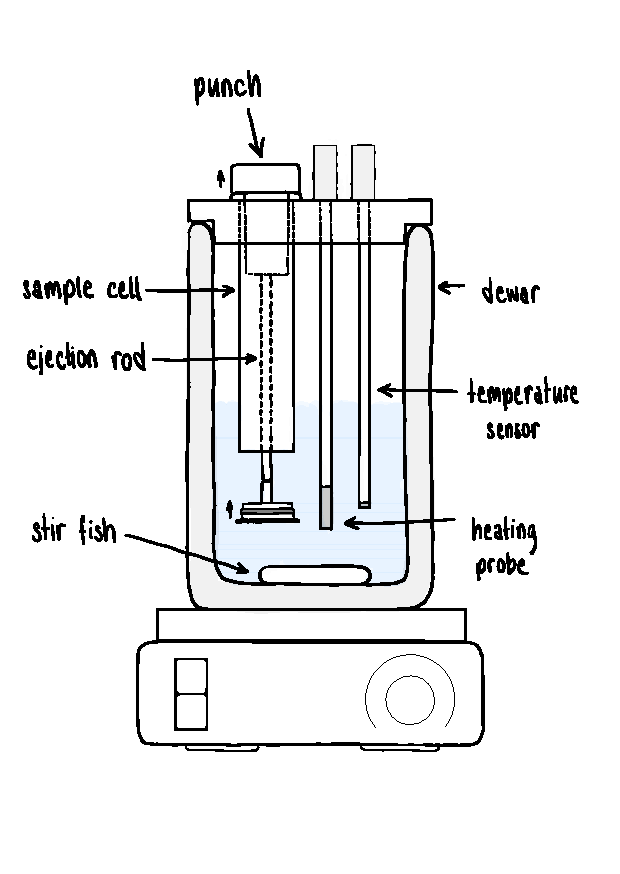
\includegraphics[width=.5\textwidth]{figures/Calorimeter.pdf}
    \caption{The entire setup for calorimetric measurements, including the \texttt{LAUDA MT} circulation thermostat, the \texttt{KNICK SE 204} measuring cell and the \texttt{KNICK Conductometer 703}.}
    \label{fig:sketch_calorimeter}
\end{figure}


\subsubsection{Calibration of the calorimeter}

\qty{100}{\milli\liter} of deionised water were measured in a volumetric flask and transferred into a \texttt{KGW ISOTHERM FB3 450mL} dewar vessel. (Fig. \ref{fig:sketch_calorimeter}) The temperature of the sample was measured under constant light stirring,  using an insertable \texttt{NATIONAL LM35 } temperature sensor with a resolution better than \qty{0.001}{\kelvin}. After waiting for the temperature to even out and recording  $T_{\mathrm{initial}}$, a constant heat supply to the system was induced by activating the heating element (\texttt{ELEKTRO-AUTOMATIK EA-3002L} for exactly \qty{120}{\second}. The power delivered was constant at $\qty{10.1}{\volt} * \qty{1.61}{\ampere} = \qty{16.26}{\watt}$ for this and all following measurements. The resulting temperature was noted down and the respective difference in temperature calculated. 

%\newpage

\subsubsection{Specific heat capacity of ethanol/water mixtures}

The same procedure was repeated for various ethanol/water solutions, whereby each team was assigned three samples of different concentration. 
 For the \qty{80}{\percent} ethanol solution \qty{72.5}{\gram} of ethanol were weighed in a previously tared beaker.  \qty{17.98}{\gram} of deionised water were added and \qty{100}{\milli\liter} of the resulting solution were measured in a volumetric flask and transferred to the dewar to be heated. 
  Similarly, \qty{90}{\gram} of ethanol and \qty{11.28}{\gram} of deionised water were used to create the \qty{90}{\percent} solution and \qty{98.72}{\gram} of ethanol and \qty{6.6}{\gram} of deionised water were used to create the \qty{95}{\percent} solution. The dewar was rinsed thorougly with deionised water before each new measurement.


\subsubsection{Solution enthalpy of ammonium nitrate}

 For the next experiment \qty{100}{\milli\liter} of deionised water were measured in a volumetric flask and transferred to the dewar. \qty{600}{\milli\gram} of \ce{NH_4NO_3}, crushed beforehand using a mortar, were weighed on a \texttt{METTLER TOLEDO AB 204} analytical balance and transferred to the bottom plate of the sample cell. The cell was closed and inserted into the lid of the dewar. The temperature recording was started and once the temperature had sufficiently equilibrated, the ammonium nitrate was released into the dewar by activating the ejection rod via the punch. (Fig. \ref{fig:sketch_calorimeter}) . Once the temperature had equilibrated once more, the system was calibrated similarly to the previous experiments by supplying heat via heating element and noting down the resulting temperature change. The experiment was repeated twice more, with \qty{595}{\milli\gram} and \qty{601}{\milli\gram} of ammonium nitrate respectively. 


\subsubsection{Calorimetric titration of vinegar} 

% Next, the concentration of acetic acid in vinegar was measured via calorimetric titration. 
Measurements in this experiment were conducted with a slightly modified calorimeter setup forgoing the probe vessel for the teflon hose of a \texttt{KNF SIMDOS 10} membrane  dosing pump. 
 \qty{25}{\milli\liter} of vinegar were measured via volumetric pipette and transferred to a volumetric flask to be filled up to \qty{100}{\milli\liter} and transferred to the dewar. 
 The dosing pump containing a \qty{1}{M} \ce{NaOH} solution was set to continuous flow of \qty{40}{\milli\liter} within \qty{3}{\minute} and the temperature was recorded during this time. 
 The experiment was repeated with a non-continuous-flow pump setting, instead opting to dose out \qty{2}{\milli\liter} within \qty{5}{\second} every \qty{20}{\second}.


\subsubsection{Melting enthalpy of ice and ice water}

The calorimeter setup in this last experiment consisted only of the dewar, its lid and the temperature sensor.
\qty{100}{\milli\liter} of deionised water were measured in a volumetric flask and transferred to the dewar and $T_{\mathrm{initial}}$ measured. A beaker with ice water was prepared and its weight together with that of an empty \qty{20}{\milli\liter} volumetric pipette measured via analytical balance. The pipette was then used to rapidly transfer \qty{20}{\milli\liter} of ice water to the dewar. The weight of the same beaker and pipette were measured again and the difference to its initial weight, equivalent to the mass of the ice water added, recorded at \qty{18.4}{\gram}. $T_{\mathrm{final}}$ was measured once the temperature had dropped significantly. The experiment was repeated twice more, using \qty{17.5}{\gram} and \qty{18.1}{\gram} of water respectively.

Following the same procedure, but with ice cubes instead of ice water, the measurement was repeated three times. A petri dish was lined with paper towels, placed on an analytical balance, several ice cubes transferred to it and the weight recorded. Using plastic forceps dry ice cubes were transferred to the dewar, until the resulting weight difference was approximately equal to the mass of the ice water added previously. By this method, the mass of the added ice cubes was measured at \qty{14.34}{\gram}, \qty{17.71}{\gram} and \qty{17.55}{\gram} respectively. 



% \subsection{}

